\documentclass[main.tex]{subfiles}
\begin{document}
\subsection{AST Transformations}
Minipass terms are subjected to several transformations before emitting
an Overpass query. Since type information is used almost everywhere,
the term is first converted into a type-tagged term (see \cref{def:ttag})
and all transformations (including translation to Overpass) are applied
afterwards.

There are three type-systems in use:
\begin{itemize}
    \item The bare Minipass type system, as described in \cref{sec:minipassbasetypes}
    \item An expert-defined type system, defined in \code{.ccg} files
        by subtyping existing Minipass types (as in \cref{sec:definingtypes})
    \item An Intermediate type system which contains more Overpass-centric
        information and facilitates translation into Overpass, which
        also subsumes the bare type system
\end{itemize}

A Minipass term, after being extracted from a CCG derivation tree, is converted
to a type-tagged term for easier manipulation and is then subjected to type
inference. Afterwards, the expert-defined type information is discarded
by squashing the extra types (see \cref{prop:makesquashfun}), which gives
a regular Minipass type-tagged term, and then setting the type system to
the Intermediate type system. This operation does not change the term, since
bare Minipass types are also types within the Intermediate type system.
Then, several optimisations (some of which take advantage of the extra type
information) are performed, and the term is finally translated to Overpass.
An illustration of this process is shown at \cref{fig:typesystems}.

\cfigure{
    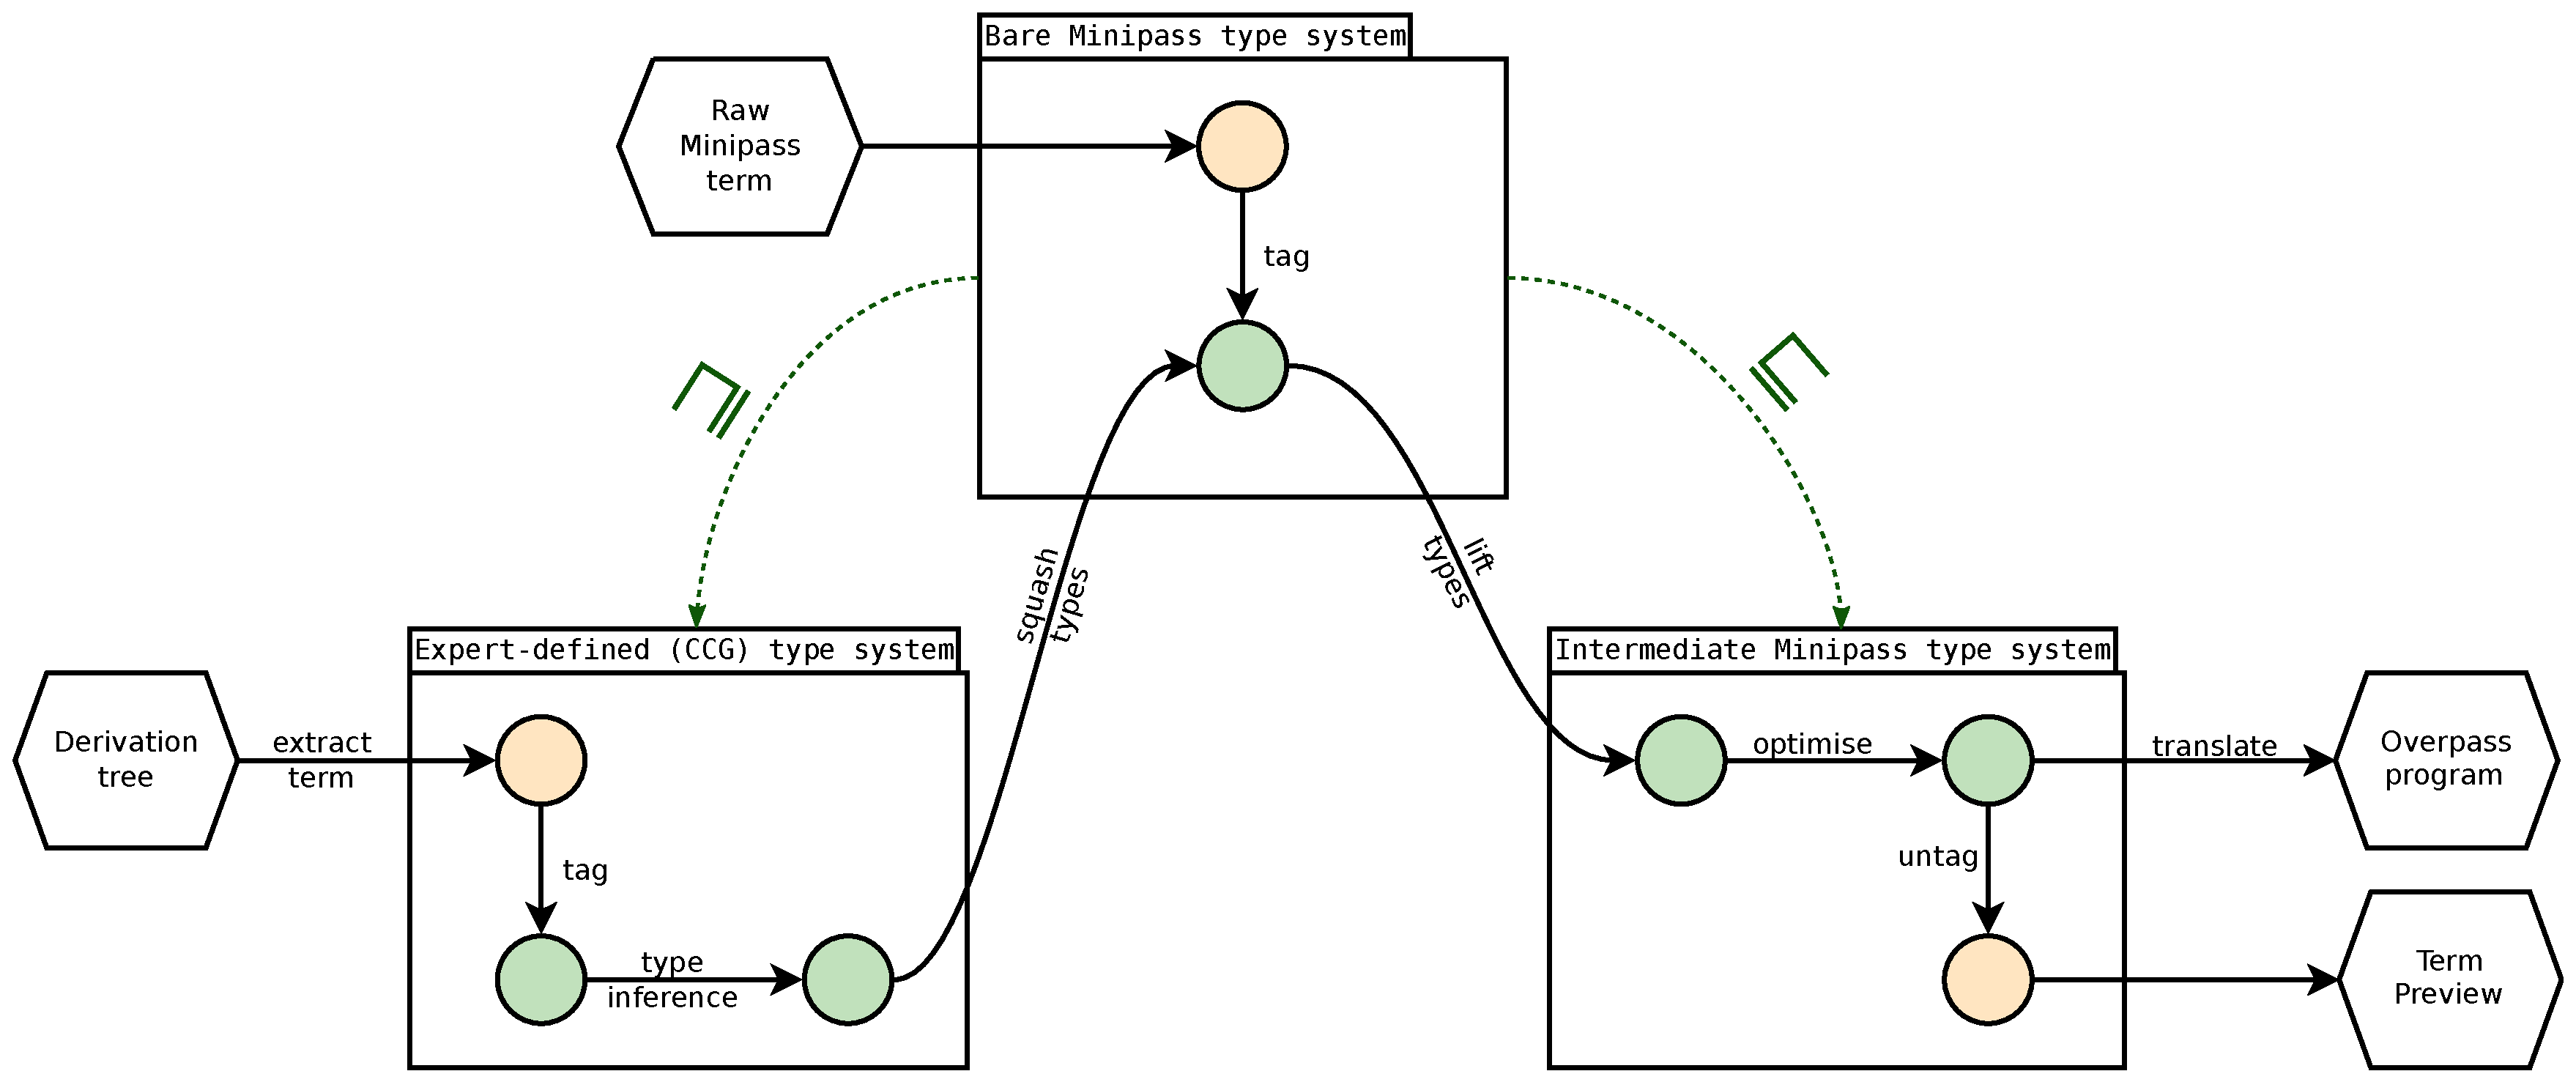
\includegraphics[width=\textwidth]{optimisation.eps}
    \caption{Illustration of the transformations undergone by a Minipass term}
    \label{fig:typesystems}
}

\subsubsection{Type inference}
\label{sec:typeinf}
Minipass allows for the usage of the special type \code{*} that acts as a
wildcard type. It violates the partial order of the type lattice since it is
equivalent to all types (i.e. $\forall \sigma \in T: (\text{\code{*}} \less \sigma)
\& (\sigma \less \text{\code{*}})$).

Thus, all significant\footnote{
    Since we only work with closed terms, the only case when a type cannot be
    inferred is when a bound variable is unused (for example in terms like
    \code{(\textbackslash x, y => y) 42}, where the type of \code{x} cannot be inferred).
    This, however, is harmless, because the type is unneeded anyway.
} occurrences of $\code{*}$ are removed by finding the fixed point of
$\mcf{propagate}$ from \cref{def:propagation}
with the following unifier:
\[
    \sigma \unify \tau =
    \begin{cases*}
        \tau ,& $\sigma = \text{\code{*}}$, \\
        \sigma ,& $\tau = \text{\code{*}}$, \\
        \sigma ,& $\sigma = \tau$, \\
        (\sigma' \unify \tau') \tot (\sigma'' \unify \tau''), &
            $\sigma = (\sigma' \tot \sigma''), \tau = (\tau' \tot \tau'')$, \\
        \lnot ! ,& $\mathsf{otherwise}$. \\
    \end{cases*}
\]

Whenever the algorithm encounters a case where the unifier is not defined,
a type error is produced.

This unifier is monotonic (\cref{def:mono}) for the partial order ``\code{*} is
above every other type, and there are no other edges''. By \cref{prop:propagateterminates},
the process of iteratively applying $\mcf{propagate}$ always terminates.
\fixednote{ако говориш за propagate, е хубаво да се докаже по-формално}

\pagebreak
\subsubsection{Minipass query optimisation}
\label{sec:optimisation}
While Overpass differentiates between 4 types of objects (nodes, ways, relations,
areas\footnote{
    The ``area'' type is only present in Overpass (not in OpenStreetMap
    databases), and \emph{area} objects are constructed by finding \emph{relations}
    that form a closed polygon \cite{overpass}.
}), its queries are heterogeneous.

\begin{mexample}
For example, the following Minipass
query\footnote{
    Minipass queries presented here assume the library from \cref{stdlib}
    for clarity.
} returns all items with name ``Brussels'':
\begin{lstwrap}\begin{lstlisting}
    name 'Brussels'
\end{lstlisting}\end{lstwrap}
The returned set, among any other objects, contains:
\begin{itemize}
    \item the city Brussels (a \emph{node})
    \item the administrative area of the city Brussels (an \emph{area})
    \item the Brussels boulevard in Sofia (a \emph{way})
\end{itemize}
Since Overpass contains separate keywords for querying different objects,
the above Minipass term would have to be translated to a query as such:
\begin{lstwrap}\begin{lstlisting}
    ( node["name" = "Brussels"];
      way["name" = "Brussels"];
      rel["name" = "Brussels"];
      area["name" = "Brussels"]; ) -> .x1;

    .x1 out;
\end{lstlisting}\end{lstwrap}
In fact, since the current implementation of \code{name} looks for the
name in several fields, the actual emitted Overpass translation is the
following:
\begin{lstwrap}\begin{lstlisting}
    ( node["name" = "Brussels"];
      way["name" = "Brussels"];
      rel["name" = "Brussels"];
      area["name" = "Brussels"];

      node["int_name" = "Brussels"];
      way["int_name" = "Brussels"];
      rel["int_name" = "Brussels"];
      area["int_name" = "Brussels"];

      node["name:en" = "Brussels"];
      way["name:en" = "Brussels"];
      rel["name:en" = "Brussels"];
      area["name:en" = "Brussels"]; ) -> .x1;

    .x1 out;
\end{lstlisting}\end{lstwrap}

Now, regard the following Minipass term:
\begin{lstwrap}\begin{lstlisting}
    in (name 'Brussels')
\end{lstlisting}\end{lstwrap}
In order to translate it, we could take the result from the previous query
and take all nodes, ways or relations\footnote{In Overpass, an \emph{area} may
    not be inside another \emph{area}} inside returned items by using the
\code{area.} filter:
\begin{lstwrap}\begin{lstlisting}
    ( node["name" = "Brussels"];
      way["name" = "Brussels"];
      rel["name" = "Brussels"];
      area["name" = "Brussels"]; ) -> .x1;

    ( node(area.x1); way(area.x1); rel(area.x1); ) -> .x2;
    .x2 out;
\end{lstlisting}\end{lstwrap}
However, the \code{area.} filter only takes into account areas from the
input set and discards all other objects. Thus, a less naïve translator should
only take areas in the first place:
\begin{lstwrap}\begin{lstlisting}
    ( area["name" = "Brussels"]; ) -> .x1;
    ( node(area.x1); way(area.x1); rel(area.x1); ) -> .x2;
    .x2 out;
\end{lstlisting}\end{lstwrap}
\end{mexample}

To make this task of optimisation easier, the Intermediate type system extends the $GSet$
type with subtypes for each combination of node, way, relation and area
(shown at \cref{fig:lattice}): essentially, we attach a set of tags (subset
of $\{ n, w, r, a \}$) to each $GSet$ type.
\cfigure{
    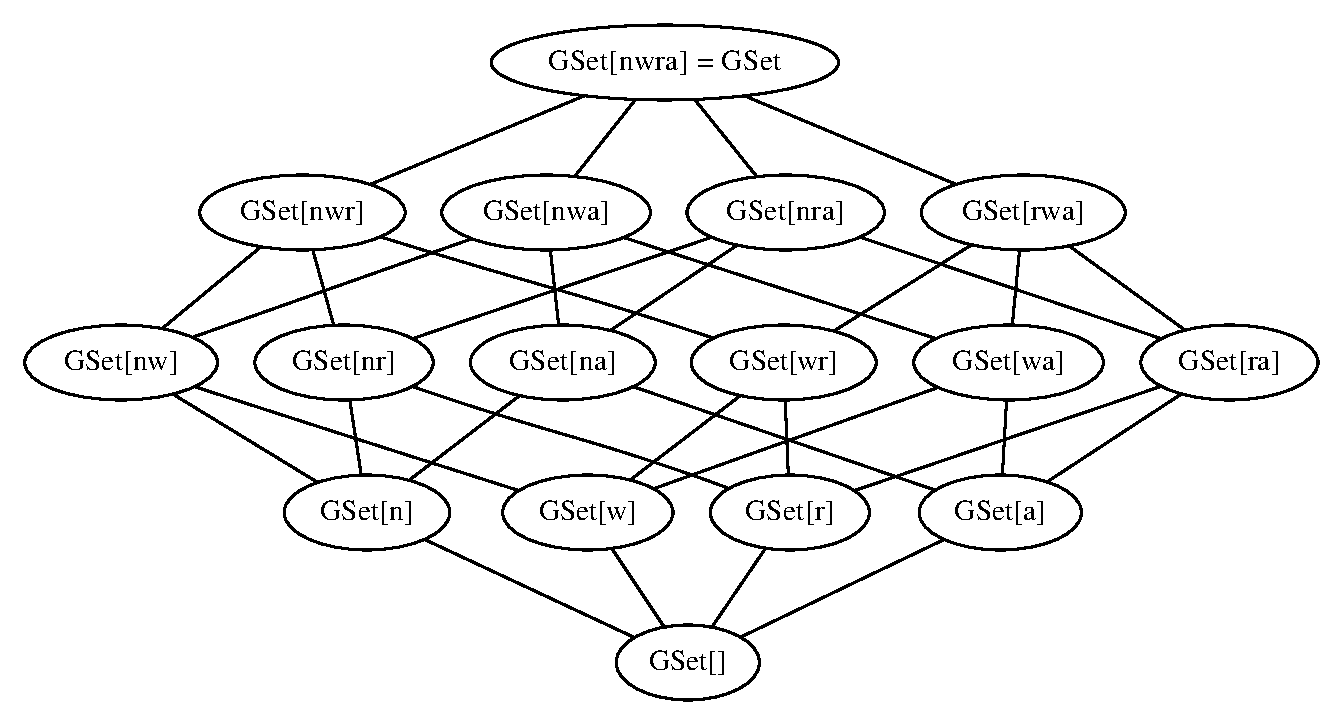
\includegraphics[width=\textwidth]{lattice.eps}
    \caption{The lattice of the $GSet$ type within the Intermediate type system}
    \label{fig:lattice}
}

During the optimisation phase, several rules are applied to each subterm, some of which are displayed in the table below:\footnote{
    In this table, ``the type of something'' means its type tag.
}:
\begin{center}
\begin{tabular}{|p{0.45\textwidth}|p{0.45\textwidth}|}
    \hline
    Subterm & Action \\
    \hline
    ``and'' of type $GSet[X] \tot GSet[Y] \tot GSet[Z]$
        & set its type to $GSet[X \cap Y \cap Z] \tot GSet[X \cap Y \cap Z] \tot GSet[X \cap Y \cap Z]$ \\
    \hline
    ``or'' of type $GSet[X] \tot GSet[Y] \tot GSet[Z]$
        & set its type to $GSet[X \cap Z] \tot GSet[Y \cap Z] \tot GSet[(X \cup Y) \cap Z]$ \\
    \hline
    $\beta$-redex & reduce it \\
    \hline
    ``get all nodes'' & change it to ``get everything'' of type $GSet[n]$ \\
    ``get all ways'' & change it to ``get everything'' of type $GSet[w]$ \\
    ``get all relations'' & change it to ``get everything'' of type $GSet[r]$ \\
    ``get all areas'' & change it to ``get everything'' of type $GSet[a]$ \\
    \hline
    ``next'' of type $GSet[X] \tot GSet[Y]$ applied to an ``in'' label
        & set its type to $GSet[X \cap \{ a \}] \tot GSet[Y \cap \{ n, w, r \}]$ \\
    \hline
    ``or'' with one of the arguments being of type $GSet[]$
        & rewrite the term to only the other argument \\
    \hline
    ... & ... \\
    \hline
\end{tabular}
\end{center}

After applying these rules, types are propagated through the term
(see \cref{def:propagation}) with the following unifier:
\[
    \sigma \unify \tau \defeq
    \begin{cases*}
        GSet[X \cap Y] ,& $\sigma = GSet[X], \tau = GSet[Y]$, \\
        Num ,& $\sigma = Num, \tau = Num$, \\
        String ,& $\sigma = String, \tau = String$, \\
        List ,& $\sigma = List, \tau = List$, \\
        (\sigma' \unify \tau') \tot (\sigma'' \unify \tau''), &
        $\sigma = (\sigma' \tot \sigma''), \tau = (\tau' \tot \tau'')$, \\
        \lnot ! ,& $\mathsf{otherwise}$. \\
    \end{cases*}
\]

We can induce a natural ordering on the finite set of $GSet$ subtypes,
so the iterative application of $\mcf{propagate}$ terminates by
\cref{prop:propagateterminates}.

It can also be seen that the optimisation rules shown above converge after
a finite number of steps. A rigorous proof will be omitted\footnote{
    As with the optimisation steps of most compilers, any bugs in the optimiser
    are left to the user to discover.
}

\fixednote{това е второто такова разсъждение. Може би имаш нужда от някаква лема от вида: ако унификаторът е еди какъв си, то неподвижната точка на propagate изисква краен брой стъпки}, which is now ready for the translation phase.

\greenbox{
    While there are many other possible optimisations which can be done here,
    only these few have been implemented as a proof-of-concept, since this
    is not the main focus of this work.
}

\subsubsection{Translating to Overpass}\label{sec:translation}
The implemented translator can only translate closed terms of non-arrow types.
It keeps an internal state which contains the statements generated thus far
and the index of the last used variable (used for generating new variable
names).
At its core is the \code{translate} function, which takes a Minipass term,
returns a \code{Value} and updates the internal state.

\code{Value} is defined as follows:
\begin{lstwrap}\begin{lstlisting}
data Value
    = StringValue Text
    | NumValue    Float
    | SetValue    VarName
    | ListValue   [ListC]

data ListC
    = NumC        Float
    | StringC     Text
    | ListC       [ListC]

type VarName = Text
\end{lstlisting}\end{lstwrap}

As can be seen above, values of type $GSet$ (\code{SetValue}) are represented
as a variable name. All other values are represented internally (this means
that they are evaluated during translation).

Here is an outline of the basic translation process:
\begin{itemize}
    \item Uncurry\footnote{See \cref{betacurry}} the term in order to be able
        to inspect its arguments
    \item Recursively evaluate (translate) all arguments
        (since there are no constants of higher-order
        type and the term has been fully $\beta$-reduced, the head
        is always a constant and the arguments are of non-arrow types ---
        see \cref{prop:simpleargs}
        \fixednote{защо аргументите не може да са стрелки?})
    \item Perform pattern matching of the argument list against a set of
        translation rules. Modify state and return value according to matched
        rule (or throw translation error).
\end{itemize}

Here are some of the aforementioned rules:
\newcounter{RuleCounter}
\newcommand\RuleCnt{\refstepcounter{RuleCounter}\theRuleCounter}
\begin{center}
\begin{tabular}{|r|p{0.45\textwidth}|p{0.45\textwidth}|}
    \hline
    \# & Input term & Action \\
    \hline
    \RuleCnt & \syntax{<string-literal>} & return a \code{StringValue} with the literal's
        content \\
    \hline
    \RuleCnt & \syntax{<number-literal>} & return a \code{NumValue} with the literal's
        content \\
    \hline
    \RuleCnt & \code{ConsString} \syntax{<arg1>} \syntax{<arg2>} & Unpack the \code{StringValue}
        returned by the translation of \syntax{<arg1>} and prepend it to the
        \code{ListValue} returned by the translation of \syntax{<arg2>} \\
    \hline
    \RuleCnt & \code{ConsNum} \syntax{<arg1>} \syntax{<arg2>} & similar to the above \\
    \hline
    \RuleCnt & \code{ConsList} \syntax{<arg1>} \syntax{<arg2>} & similar to the above \\
    \hline
    \RuleCnt \label{rule:filter} & ``and'', ``or'', ``get'' or ``next'', applied to its respective arguments &
        Walk the syntax tree of ``and''s and ``or''s downwards, stopping at
        leaves (anything that is not ``and'' or ``or''). Create an Overpass
        filter from the resulting tree. Generate a new variable name and emit
        an Overpass statement that saves the result from the filter into the
        variable. Return a \code{SetValue} bearing said variable name. \\
    \hline
\end{tabular}
\end{center}

At the end of translation, if the result is a \code{SetValue}, an overpass
``\code{out .<variable>;}'' statement is added.

\begin{mexample}
    Consider the following query, generated by the query ``pharmacies in Sofia'':
    \begin{lstwrap}\begin{lstlisting}
        and (get (consString 'tagFilter' (consList (consString '=' (consString 'amenity' (consString 'pharmacy' empty))) empty))) (next (consString 'in' empty) (or (or (get (consString 'tagFilter' (consList (consString '=' (consString 'name' (consString 'Sofia' empty))) empty))) (get (consString 'tagFilter' (consList (consString '=' (consString 'int_name' (consString 'Sofia' empty))) empty)))) (get (consString 'tagFilter' (consList (consString '=' (consString 'name:en' (consString 'Sofia' empty))) empty)))))
    \end{lstlisting}\end{lstwrap}
    Since long labels make this code rather unreadable, we will replace them
    by human-readable placeholders, and will assign numbers to AST nodes
    (after uncurrying):
    \begin{lstwrap}\begin{lstlisting}
        and                                     -- #1
            (get                                -- #2
                <amenity=pharmacy>)             -- #3
            (next                               -- #4
                <in>                            -- #5
                (or                             -- #6
                   (or                          -- #7
                        (get                    -- #8
                            <name=Sofia>)       -- #9
                        (get                    -- #10
                            <int_name=Sofia>)   -- #11
                    )
                    (get                        -- #12
                        <name:en=Sofia>)        -- #13
                )
            )
    \end{lstlisting}\end{lstwrap}

    The translator will first apply rule \ref{rule:filter} on the following
    syntax tree:
    \centree{
        .{ \code{and\#1} }
            [ .{ \code{get\#2} } ]
            [ .{ \code{next\#4} } ]
    }

    For this tree, after recursively translating the \code{amenity\#3},
    \code{in\#5} and \code{or\#6} subterms, the translator
    would emit the following Overpass filter:
    \begin{lstwrap}\begin{lstlisting}
        ( node(area.<result from or#6>)["amenity" = "pharmacy"]; ) -> .<newvar>;
    \end{lstlisting}\end{lstwrap}

    So, let's see how \code{or\#6} will be evaluated. Again, we apply
    rule \ref{rule:filter} on the following syntax tree:
    \centree{
        .{ \code{or\#6} }
            [ .{ \code{or\#7} }
                [ .{ \code{get\#8} } ]
                [ .{ \code{get\#10} } ]
            ]
            [ .{ \code{get\#12} } ]
    }

    After recursively translating \code{name\#9}, \code{int\_name\#11}
    and \code{name:en\#13}, the translator emits this\footnote{
        Only ``area'' nodes are emitted because the type of the ``get''s has
        been inferred as $GSet[a]$ by the optimiser.
    } Overpass filter:

    \begin{lstwrap}\begin{lstlisting}
        ( area["name" = "Sofia"];
          area["int_name" = "Sofia"];
          area["name:en" = "Sofia"];   ) -> <newvar>;
    \end{lstlisting}\end{lstwrap}

    Finally, after substituting the generated variable names and adding
    an output statement, we get the following query:

    \begin{lstwrap}\begin{lstlisting}
        ( area["name" = "Sofia"];
          area["int_name" = "Sofia"];
          area["name:en" = "Sofia"];   ) -> .x1;
        ( node(area.x1)["amenity" = "pharmacy"]; ) -> .x2;
        out .x2;
    \end{lstlisting}\end{lstwrap}
\end{mexample}

While this translator is at proof-of-concept level, it can easily be extended
to cover most of Overpass. An overview of features is presented in
\cref{table:overpassfeatures}.

\begin{samepage}
\begin{table}[h]
    \begin{center}
        \begin{tabular}{|r|l|}
            \hline
            Feature & Status \\
            \hline
            Set Union & Implemented \\
            Set Intersection & Implemented \\
            Set Difference & Trivial to implement \\
            Set Negation & Easy to implement\footnote{
                Negation must be converted to set difference whenever possible
                because it requires enumerating the entire dataset in most
                implementations \cite{overpass}
            }    \\
            Equality filter & Implemented \\
            Regex filter & Implemented \\
            Bounding box & Trivial to implement \\
            Recurse (get children) & Trivial to implement \\
            Get item by id & Trivial to implement \\
            Around (within distance) & Implemented \\
            Area (within area) & Implemented \\
            Relation operators (next, previous) & Trivial to implement \\
            Recurse (get children) & Trivial to implement \\
            For-each-loop & Difficult to implement \\
            Complete (fixed point) & Easy to implement \\
            Retro & Not applicable\footnote{``Retro'' deals with the map's edit
                history} \\
            Counting, summing, stats etc & Difficult to implement \\
            ... & ... \\
            \hline
        \end{tabular}
    \end{center}
    \caption{Some Overpass features and their corresponding level of support by the translator}
    \label{table:overpassfeatures}
\end{table}
\end{samepage}
\end{document}
